% ===================================================================
%  CPE 333 Operating Systems -- Problem Session 10
%  The Dining Philosophers vs. The Cigarette Smokers
%
%  BUILD:   powershell -ExecutionPolicy Bypass -File ..\scripts\build_pdf.ps1
%
%  The sheet asks for 4-7 content pages, not counting the cover and the
%  references: frames 2-8 are the content, frame 9 the references.
% ===================================================================
\documentclass[aspectratio=169,11pt]{beamer}
% Beamer setup for PS10. Hand-edited.
\usepackage[T1]{fontenc}
\usepackage{lmodern}
\usepackage{booktabs}
\usepackage{array}
\usepackage{listings}
\usepackage{xcolor}

% The sheet's own colours: philosophers in red, smokers in blue.
\definecolor{phil}{HTML}{C00000}
\definecolor{smok}{HTML}{0070C0}
\definecolor{ink}{HTML}{222222}
\definecolor{muted}{HTML}{666666}
\definecolor{codebg}{HTML}{F4F4F4}

\usetheme{default}
\setbeamertemplate{navigation symbols}{}
\setbeamercolor{normal text}{fg=ink}
\setbeamercolor{frametitle}{fg=ink}
\setbeamercolor{structure}{fg=smok}
\setbeamerfont{frametitle}{size=\large,series=\bfseries}
\setbeamertemplate{itemize items}{\textbullet}
\setbeamertemplate{footline}{%
  \hfill{\scriptsize\color{muted}\insertframenumber\ /\ \inserttotalframenumber}\hspace{1.2em}\vspace{0.8em}}

\newcommand{\Smk}{\textcolor{smok}{\textbf{Cigarette Smokers}}}
\newcommand{\Dph}{\textcolor{phil}{\textbf{Dining Philosophers}}}

\lstdefinestyle{pseudo}{
  basicstyle=\ttfamily\scriptsize,
  backgroundcolor=\color{codebg},
  frame=none,
  xleftmargin=0.4em, xrightmargin=0.4em,
  aboveskip=0.3em, belowskip=0.3em,
  columns=fullflexible, keepspaces=true,
  keywordstyle=\bfseries,
  morekeywords={if,elif,else,while,return,void,int},
  commentstyle=\color{muted}\itshape,
  morecomment=[l]{//},
}
\lstset{style=pseudo}


\begin{document}

% ------------------------------------------------------------- cover ---
{\setbeamertemplate{footline}{}
\begin{frame}
  \centering
  \vspace{1.2em}
  {\small\color{muted} CPE 333 Operating Systems, 1/2026 \quad\textbullet\quad Problem Session 10}\\[1.6em]
  {\LARGE\bfseries\textcolor{phil}{The Dining Philosophers}\\[0.3em]
   {\large\mdseries vs.}\\[0.3em]
   \textcolor{smok}{The Cigarette Smokers}}\\[2.2em]
  \begin{tabular}{@{}l@{\hspace{2em}}l@{}}
    Kiatisak Markmeeshap & 67070501005 \\
    Tithinan Sobking     & 67070501018 \\
    Worawut Sereethai    & 67070501040 \\
    Chanya Poolketkij    & 67070501058
  \end{tabular}
\end{frame}
}

% ------------------------------------------------------ 1. the problem ---
\begin{frame}[fragile]{The \Smk{} problem (Patil, 1971)}
  \begin{columns}[T]
    \begin{column}{0.54\textwidth}
      \small
      \begin{itemize}
        \item Making a cigarette needs \textbf{tobacco}, \textbf{paper} and \textbf{matches}.
        \item Three smokers each hold an unlimited supply of \emph{one} ingredient.
        \item An \textbf{agent} (a dealer that supplies ingredients, like
              the OS) holds all three. It repeatedly puts two different
              ingredients on the table, then waits for a smoker to finish.
        \item The smoker holding the third ingredient should take both, smoke,
              and wake the agent.
        \item \textbf{Constraint:} the agent's code is fixed; only the
              smokers may be written.
      \end{itemize}
      \vspace{0.3em}
      {\footnotesize Patil posed it to argue that semaphores (P/V) are too weak
      to solve it without conditional statements~[1].}
    \end{column}
    \begin{column}{0.42\textwidth}
      {\footnotesize\color{muted} Agent, as given (one of three; the others
      supply the other two pairs)~[3]}
\begin{lstlisting}
agentSem = Semaphore(1)
tobacco = Semaphore(0)
paper   = Semaphore(0)
match   = Semaphore(0)

// Agent A
agentSem.wait()
tobacco.signal()
paper.signal()
\end{lstlisting}
      {\footnotesize\color{muted} Agents B and C signal
      \texttt{paper}+\texttt{match} and \texttt{tobacco}+\texttt{match}.}
    \end{column}
  \end{columns}
\end{frame}

% ------------------------------------------- 2. the obvious attempt ---
\begin{frame}[fragile]{Why the obvious solution deadlocks}
  \label{naive}
  \begin{columns}[T]
    \begin{column}{0.40\textwidth}
\begin{lstlisting}
// smoker with matches
tobacco.wait()
paper.wait()
agentSem.signal()

// smoker with paper
tobacco.wait()
match.wait()
agentSem.signal()

// smoker with tobacco
paper.wait()
match.wait()
agentSem.signal()
\end{lstlisting}
    \end{column}
    \begin{column}{0.56\textwidth}
      \small
      \textbf{Interleaving.} The agent puts out \emph{tobacco + paper}
      (meant for the matches smoker).
      \begin{enumerate}
        \item The \emph{paper} smoker takes the tobacco, then blocks on \texttt{match}.
        \item The \emph{tobacco} smoker takes the paper, then blocks on \texttt{match}.
        \item The \emph{matches} smoker blocks on \texttt{tobacco}; the agent blocks on \texttt{agentSem}.
      \end{enumerate}
      No one can proceed: a \textbf{deadlock}~[3].
      \vspace{0.5em}

      Each semaphore says only ``this ingredient is here''. A smoker
      cannot tell whether an ingredient is meant for it until it has
      seen \emph{both}, so it grabs one and holds it while waiting
      (\emph{hold and wait}).
    \end{column}
  \end{columns}
\end{frame}

% ----------------------------------------------------- 3. pushers ---
\begin{frame}[fragile]{A solution: pushers decide who smokes}
  \begin{columns}[T]
    \begin{column}{0.53\textwidth}
\begin{lstlisting}
mutex = Semaphore(1)
isTobacco = isPaper = isMatch = False
tobaccoSem = paperSem = matchSem = Semaphore(0)

// Pusher A: one per ingredient
tobacco.wait()
mutex.wait()
if isPaper:
    isPaper = False
    matchSem.signal()
elif isMatch:
    isMatch = False
    paperSem.signal()
else:
    isTobacco = True
mutex.signal()

// smoker with tobacco
tobaccoSem.wait()
makeCigarette(); agentSem.signal(); smoke()
\end{lstlisting}
    \end{column}
    \begin{column}{0.44\textwidth}
      \small
      \begin{itemize}
        \item A helper thread (\emph{pusher}) waits on each ingredient
              semaphore and records it in shared state under a mutex.
        \item The pusher that sees the \emph{second} ingredient knows the pair,
              and signals exactly the one smoker that can use it.
        \item Smokers wait on a single semaphore, so none ever holds a
              partial pair. The agent is unchanged.
      \end{itemize}
      \vspace{0.3em}
      {\footnotesize Downey's form~[3]. Parnas showed Patil's claim holds
      only under strong restrictions on P and V, and solved the problem
      without conditionals~[2].}
    \end{column}
  \end{columns}
\end{frame}

% --------------------------------------- 4. dining philosophers recap ---
\begin{frame}[fragile]{The \Dph{} (Dijkstra, 1971)}
  \begin{columns}[T]
    \begin{column}{0.49\textwidth}
      \small
      \begin{itemize}
        \item Five philosophers alternate between thinking and eating;
              one fork lies between each pair.
        \item Eating needs both the left and the right fork.
        \item If all five take their left fork at once, each waits forever
              for the right one: a \textbf{circular wait}~[4],~[6].
        \item Standard fixes~[3],~[5],~[6]:
          \begin{itemize}
            \item order the forks (one philosopher takes the right first);
            \item seat at most four at a time;
            \item take both forks only when both are free (Dijkstra's
                  state-based solution).
          \end{itemize}
      \end{itemize}
    \end{column}
    \begin{column}{0.48\textwidth}
      % The naive deadlock: P_p holds fork p (solid) and waits for fork p+1
      % (dashed). Fork p sits between P_{p-1} and P_p.
      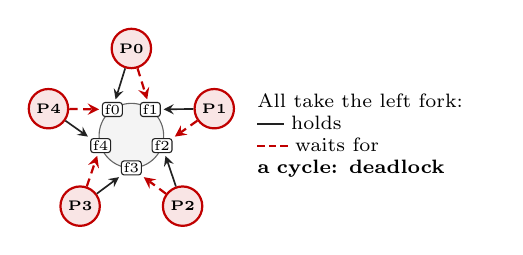
\begin{tikzpicture}[scale=0.41,>=stealth,
          phil/.style={circle,draw=phil,fill=phil!10,thick,minimum size=5mm,
                       inner sep=0pt,font=\tiny\bfseries},
          fork/.style={rectangle,rounded corners=1pt,draw=ink,fill=white,
                       inner sep=0.8pt,font=\tiny}]
        \draw[draw=muted,fill=codebg] (0,0) circle (1.0);
        \foreach \p in {0,...,4} {
          \node[phil] (P\p) at ({90-72*\p}:2.7) {P\p};
          \node[fork] (F\p) at ({126-72*\p}:1.0) {f\p};
        }
        \foreach \p in {0,...,4} {
          \pgfmathtruncatemacro{\q}{mod(\p+1,5)}
          \draw[->,semithick,ink,shorten >=1pt] (P\p) -- (F\p);
          \draw[->,semithick,densely dashed,phil,shorten >=1pt] (P\p) -- (F\q);
        }
        \node[anchor=west,align=left,font=\scriptsize,text width=2.9cm]
          at (3.6,0) {All take the left fork:\\
            \textcolor{ink}{\rule[0.5ex]{1.2em}{0.8pt}} holds\\
            \textcolor{phil}{\rule[0.5ex]{0.35em}{0.8pt}\,\rule[0.5ex]{0.35em}{0.8pt}\,\rule[0.5ex]{0.35em}{0.8pt}} waits for\\
            \textbf{a cycle: deadlock}};
      \end{tikzpicture}

      {\footnotesize\color{muted} Breaking the circular wait (Lecture~10)~[6]}
\begin{lstlisting}
int left(int p)  { return p; }
int right(int p) { return (p + 1) % 5; }

void getforks(int p) {
    if (p == 4) {
        sem_wait(&forks[right(p)]);
        sem_wait(&forks[left(p)]);
    } else {
        sem_wait(&forks[left(p)]);
        sem_wait(&forks[right(p)]);
    }
}
\end{lstlisting}
    \end{column}
  \end{columns}
\end{frame}

% ------------------------------------------------- 5. comparison table ---
\begin{frame}{The two problems side by side}
  \footnotesize
  \renewcommand{\arraystretch}{1.25}
  \begin{tabular}{@{}>{\bfseries}p{0.17\textwidth}p{0.385\textwidth}p{0.385\textwidth}@{}}
    \toprule
    & \Dph & \Smk \\
    \midrule
    Resources      & Five forks, \emph{reusable}: returned after eating
                   & Three ingredients, \emph{consumable}: used up, then re-supplied by the agent \\
    Who needs what & Fixed: philosopher $p$ always needs forks $p$ and $p{+}1$
                   & Decided at run time by the agent's random choice of pair \\
    Symmetry       & All processes identical
                   & Three different smokers, plus an agent we may not change \\
    What we control& All of the code
                   & Only the smokers (and any helpers we add) \\
    Deadlock cause &Circular wait on forks held by neighbours
                   & Taking an ingredient meant for someone else, then waiting for one that never comes \\
    Typical fix    & Order resources, limit diners, or take both forks at once
                   & Collect the pair first, then wake the right smoker (pushers) \\
    What it teaches& Deadlock and starvation in resource allocation
                   & How expressive semaphores are; synchronising on combined state \\
    \bottomrule
  \end{tabular}
\end{frame}

% ------------------------------------- 6. why the fixes do not transfer ---
\begin{frame}{Why the philosophers' fixes do not save the smokers}
  \small
  \begin{itemize}
    \item \textbf{Resource ordering.} Order the ingredients
          tobacco $<$ paper $<$ match. The code on page~\pageref{naive} already acquires
          in that order, and it still deadlocks. Ordering breaks a cycle of
          processes \emph{holding} resources; here the missing ingredient is
          held by no one: the agent never produces it.
    \item \textbf{Acquire both atomically.} Wrapping both waits in one
          mutex (Lecture~10's hold-and-wait prevention) is worse: the first
          smoker in waits for an ingredient that is not on the table, while
          holding the mutex every other smoker needs.
    \item \textbf{What does carry over.} Dijkstra's own solution and the
          pushers share one shape: record state under a mutex, decide who
          can proceed, and signal that process's private semaphore~[3],~[4].
          The decision is made where the whole state is visible, not by each
          process grabbing one resource at a time.
  \end{itemize}
\end{frame}

% ------------------------------------------------------ 7. conclusion ---
\begin{frame}{Conclusion}
  \small
  \begin{itemize}
    \item Both problems deadlock when a process takes one resource and waits
          for a second.
    \item In the \Dph{} the second resource \emph{exists} but is held by a
          neighbour, so breaking the circular wait is enough.
    \item In the \Smk{} the second resource may \emph{never be produced} for
          that smoker, so no order of waits helps; the pair must be identified
          before anyone commits to it.
    \item The \Smk{} also fixes part of the system (the agent), which is the
          realistic case: an OS allocates resources without knowing which
          process will use them.
    \item Both are solved by the same pattern: shared state under a mutex,
          plus one semaphore per process to wake exactly the one that can run.
  \end{itemize}
\end{frame}

% ------------------------------------------------------- references ---
\begin{frame}{References}
  \scriptsize
  \begin{enumerate}
    \item[{[1]}] S.\,S. Patil, ``Limitations and capabilities of Dijkstra's
      semaphore primitives for coordination among processes,'' Computation
      Structures Group Memo~57, Project MAC, MIT, Cambridge, MA, Feb.~1971.
    \item[{[2]}] D.\,L. Parnas, ``On a solution to the cigarette smoker's
      problem (without conditional statements),'' \emph{Commun.\ ACM},
      vol.~18, no.~3, pp.~181--183, Mar.~1975, doi:10.1145/360680.360709.
    \item[{[3]}] A.\,B. Downey, \emph{The Little Book of Semaphores}, 2nd ed.,
      v2.2.1. Green Tea Press, 2016, Sec.~4.4 (Dining philosophers) and
      Sec.~4.5 (Cigarette smokers problem).
    \item[{[4]}] E.\,W. Dijkstra, ``Hierarchical ordering of sequential
      processes,'' \emph{Acta Informatica}, vol.~1, no.~2, pp.~115--138, 1971,
      doi:10.1007/BF00289519.
    \item[{[5]}] R.\,H. Arpaci-Dusseau and A.\,C. Arpaci-Dusseau,
      \emph{Operating Systems: Three Easy Pieces}, v1.10.
      Arpaci-Dusseau Books, 2023, Ch.~31 (Semaphores).
    \item[{[6]}] CPE 333 Operating Systems, Lecture~10: Resource Allocation
      and Deadlock, 1/2026, slides 9--21.
  \end{enumerate}
\end{frame}

\end{document}
